%----------------------------------------------------------------------------------------
%
% A LaTeX-template for 1DV510. Modified and translated by Björn Lindenberg at LNU.
% Based on an original master thesis template created by Marcus Wilhelmsson at LNU.
%
%----------------------------------------------------------------------------------------

% Settings and document configuration

\documentclass[a4paper,12pt]{article} 
\usepackage[T1]{fontenc} 
\usepackage{times} 
\usepackage[swedish,english]{babel} 
\usepackage[utf8]{inputenc} 
\usepackage{dtk-logos} 
\usepackage{wallpaper} 
\usepackage[absolute]{textpos} 
\usepackage[top=2cm, bottom=2.5cm, left=3cm, right=3cm]{geometry} 
\usepackage[parfill]{parskip} 
\usepackage{csquotes} 
\usepackage{float} 
\usepackage{lipsum} % Used for dummy text. Can be removed.
\usepackage{listings, color}

\lstdefinestyle{Asm}{
  belowcaptionskip=1\baselineskip,
  breaklines=true,
  frame=L,
  xleftmargin=\parindent,
  language=[x86masm]Assembler,
  showstringspaces=false,
  basicstyle=\footnotesize\ttfamily,
  keywordstyle=\bfseries\color{purple!40!black},
  commentstyle=\itshape\color{green!40!black},
  identifierstyle=\color{blue},
  stringstyle=\color{orange},
}

% Fontsizes for section headings.
\usepackage{sectsty} 
\sectionfont{\fontsize{14}{15}\selectfont}
\subsectionfont{\fontsize{12}{15}\selectfont}
\subsubsectionfont{\fontsize{12}{15}\selectfont}

%----------------------------------------------------------------------------------------
%	This part is used for the text box on the title page
%----------------------------------------------------------------------------------------
\newsavebox{\mybox}
\newlength{\mydepth}
\newlength{\myheight}

\newenvironment{sidebar}%
{\begin{lrbox}{\mybox}\begin{minipage}{\textwidth}}%
{\end{minipage}\end{lrbox}%
 \settodepth{\mydepth}{\usebox{\mybox}}%
 \settoheight{\myheight}{\usebox{\mybox}}%
 \addtolength{\myheight}{\mydepth}%
 \noindent\makebox[0pt]{\hspace{-20pt}\rule[-\mydepth]{1pt}{\myheight}}%
 \usebox{\mybox}}

%----------------------------------------------------------------------------------------
%	Title
%----------------------------------------------------------------------------------------
\newcommand\BackgroundPic{
    \put(-2,-3){
    
\includegraphics[keepaspectratio,scale=0.3]{img/lnu_etch.png} % Background image
    }
}
\newcommand\BackgroundPicLogo{
    \put(30,740){
    
\includegraphics[keepaspectratio,scale=0.10]{img/logo.png} % LNU logo
    }
}

\title{
\vspace{-8cm}
\begin{sidebar}
    \vspace{10cm}
    \normalfont \normalsize
    \huge Computer Technology I\\ % Main title
    \vspace{-1.3cm}
\end{sidebar}
\vspace{3cm}
\begin{flushleft}
    \huge Lab. 2 : Subroutines % Subtitle
     \small \\ \emph{}
\end{flushleft}
\null
\vfill
\begin{textblock}{5}(10,13)
\begin{flushright}
\begin{minipage}{\textwidth}
\begin{flushleft} \large
\emph{Author:}\textsc{ Loic GALLAND, Leonardo PEDRO}\\  % Author
\emph{Supervisor:}  \textsc{} \\  % Author
\emph{Semester:} Autumn 2019\\ % Semester
\emph{Area:} Computer Science \\ % Area
\emph{Course code:} 1DT301 % Course
\end{flushleft}
\end{minipage}
\end{flushright}
\end{textblock}
}

\date{} % Empty date command. Use \today inside for today's date.
\author{} % Normally one would use this to define authors. However in this case the title command takes care of everything, so we leave the field empty to get rid of warnings. 

\begin{document}

\pagenumbering{gobble} % Turn off page numbering
\newgeometry{left=5cm}
\AddToShipoutPicture*{\BackgroundPic} % Adds the background image to the title page
\AddToShipoutPicture*{\BackgroundPicLogo} % Adds the logo to the title page
\maketitle % Prints the title
\restoregeometry
\clearpage

\pagenumbering{roman} % Roman page numbering for abstract page


\selectlanguage{english}

\newpage

\pagenumbering{gobble} % Turn off page numbering
\tableofcontents 

\newpage
\pagenumbering{arabic} % Turn on page numbering


\section{Task 1 - Switch – Ring counter / Johnson counter}

\textit{Write a program which switch between Ring counter and Johnson counter. You should not use
Interrupt in this lab. The pushbutton must be checked frequently, so there is no delay between the
button is pressed and the change between Ring/Johnson. Use SW0 (PA0) for the button. Each
time you press the button, the program should change counter.}

\lstset{style=Asm}
\begin{lstlisting}
;>>>>>>>>>>>>>>>>>>>>>>>>>>>>>>>>>>>>>>>>>>>>>>>>>>>>>>>>>>>
; 1DT301, Computer Technology I
; Date: 2016-09-15
; Author:
; Loic GALLAND
; Leonardo PEDRO
;
; Lab number: 2
; Title: Subroutines
;
; Hardware: STK600, CPU ATmega2560
;
; Function: Program that when the Switch number 0 is pressed, it will change between the Ring Counter and the Johnson Counter.
;
; Input ports: PORTA will be used as input to be able to get the information from the switches.
;
; Output ports: PORTB will be used as output to be able to light up the LEDs in the corresponding manner.
;
; Subroutines: To be able to do the delay
; Included files: m2560def.inc
;<<<<<<<<<<<<<<<<<<<<<<<<<<<<<<<<<<<<<<<<<<<<<<<<<<<<<<<<<<<
.includes "m2560def.inc"
; Initialize SP, Stack Pointer
ldi r20, HIGH(RAMEND) ; R20 = high part of RAMEND address
out SPH,R20 ; SPH = high part of RAMEND address
ldi R20, low(RAMEND) ; R20 = low part of RAMEND address
out SPL,R20 ; SPL = low part of RAMEND address

ldi r16, 0xFF ;setting up the data direction register port B
out DDRB, r16 ;Set port B as output
ldi r16, 0x00	;Set the data direction register port A
out DDRA, r16	;Set portA as input

ldi r24, 0b11111110	;Desired switch

RC:	;Ring Counter Code
	ldi r21, 0b11111111; inital LED state
	out portB, r21	;Turn off all the lights
	mov r17, r21	;Copy r21 into r17
	ldi r22, 0xFF	;To compare to make it restart when all the lights turn off 
	RC_loop:
		out portB, r17	;Show the corresponding lights
		rol r17	;rotate the bits to make them go left
		CALL Delay1	;Delay of 0.5 seconds
		in r25, PINA	;Read the input from the switch
		cp r25,r24	;Compare the switches with the desired switch
		breq JC	;If they are =, go to Johnson Counter
		cp r17, r22		;Check if all the lights are turned off
		breq RC_light	;
	rjmp RC_loop
	RC_light:
		rol r17	;do a rol here because we are not supposed to see it appear.
		out portB, r17	;light up the desired LEDs
		rjmp RC_loop	;go back to the loop to make it continue
rjmp RC

JC:	;Johnson Counter Code
	ldi r21, 0b11111110	;r21 = to light up the LEDs 
	ldi r22, 0b11111111 ;Desired condituon
	ldi r23, 0b00000000	;Desired condition

	my_loop1:	;Loop to do the going left part of the Johnson Counter
		out portB, r21	;Light up the corresponding LEDs
		LSL r21	;Logical shift to the left of R21
		CALL Delay1	;Delay of 0.5s
		in r25, PINA	;Get the input from PINA
		cp r25,r24	;Compare input and desired switch
		breq RC	If equal go back to Ring Counter
		cp r21, r23 ;compare  info with desired one 
		breq light	;If equal go to "light" where it is going right.
	rjmp my_loop1

	light:	;initialisation process to be able to go right
		out portB, r23	;Turn on all the lights
		CALL Delay1	;Delay of 0.5s
		ldi r21, 0b10000000	;Set up the first iteration to make sure it goes right correctly 
		out portB, r21	;output to PortB
		Second_loop:	;Action of going right here
			in r25, PINA	;check info from switches
			cp r25,r24	;Compare switches with desired switch
			breq RC	;If equal go back to Ring Counter
			out portB, r21	;Output it to r21
			ASR r21	;Arithmetic Shift right to be able to shift the bits to the right.
			CALL Delay1	;Delay of 0.5s
			cp r21, r22 ;compare  info with desired one 
			breq my_loop1	;if equal go back my_loop1 and go right again
		rjmp Second_loop
rjmp JC
Delay1:
; Generated by delay loop calculator
; at http://www.bretmulvey.com/avrdelay.html
; Delay 1 950 500 cycles
; 500ms at 3.901 MHz
    ldi  r18, 10
    ldi  r19, 230
    ldi  r20, 22
L1: dec  r20
    brne L1
    dec  r19
    brne L1
    dec  r18
    brne L1
RET
\end{lstlisting}
This is the flowchart of the task 1:
\begin{center}
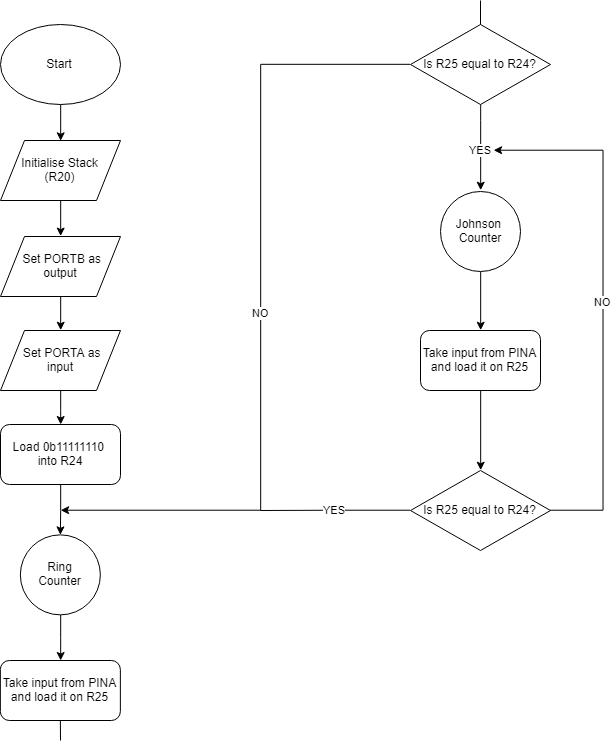
\includegraphics[scale=0.7]{img/Task1.png}
\end{center}
\newpage
\section{Task 2 - Electronic dice}
\textit{You should create an electronic dice. Think of the LEDs placed as in the picture below. The
number 1 to 6 should be generated randomly. You could use the fact that the time you press the
button varies in length.}

\lstset{style=Asm}
\begin{lstlisting}
;>>>>>>>>>>>>>>>>>>>>>>>>>>>>>>>>>>>>>>>>>>>>>>>>>>>>>>>>>>>
; 1DT301, Computer Technology I
; Date: 2016-09-15
; Author:
; Loic GALLAND
; Leonardo PEDRO
;
; Lab number: 2
; Title: Subroutines
;
; Hardware: STK600, CPU ATmega2560
;
; Function:Program that represent an electronic dice. The number 1 to 6 will be choose randomly every time we click on the button
;
; Input ports: PORTA will be used as input to get the information from the switches.
; Output ports: PORTB will be used as output to light up the LEDs when needed. 
;
; Subroutines: None needed here.
; Included files: m2560def.inc
;<<<<<<<<<<<<<<<<<<<<<<<<<<<<<<<<<<<<<<<<<<<<<<<<<<<<<<<<<<<
.include "m2560def.inc"

ldi r16, 0xFF ;setting up the data direction register PORTB
out DDRB, r16 ;Set PORTB as output

ldi r16,0x00	;setting up the data direction register PORTA
out DDRA, r16	;Set PORTA as input

ldi r19,1; Counter for the number of the dice 
ldi r25, 0xFF	;To turn off all the LEDs
out PortB,r25
ldi r24,0b11111110	;Desired Switch Binary Code

Listening_For_Switch_Press:	;Listening when the switch will be pressed.
	in r17,PINA	;Get info from switches 
	cp r17,r24	;Compare the switches and the desired switch binary code.
	breq Listening_For_Switch_Release	;If equal goes to the loop below.
rjmp Listening_For_Switch_Press

Listening_For_Switch_Release:	;Listening when the switch will be released
	inc r19	;increase r19 by 1 every time it comes into this loop
	cpi r19,7	;compare to a constant (7) as we only want numbers from 1 to 6
	breq reset	;if equal reset the counter
	in r17,PINA	;Check the info from the switches
	cp r17,r25	;Check if user has released the switches
	breq RD	;If yes go to RD loop
rjmp Listening_F	or_Switch_Release

reset:	;to reset the counter
ldi r19,1
rjmp Main

RD:	;This is where the random will happen
	cpi r19,1	;When it will be sent to this loop 
	breq ONE	;It will stop on one of those numbers
	cpi r19,2	;Depending on which number is 
	breq TWO	;r19 right now it will decide which
	cpi r19,3	;number it will gets
	breq THREE
	cpi r19,4
	breq FOUR
	cpi r19,5
	breq FIVE
	cpi r19,6
	breq SIX
rjmp RD

ONE:			;If r19 was equal to 1 it will come here
ldi r18,0b11101111	;Load to r18 the corresponding binary code to make it look like a 1
out PortB,r18		;Output it to PORTB
rjmp Listening_For_Switch_Press	;and go back to the first loop 
TWO:
ldi r18,0b10111011
out PortB,r18
rjmp Listening_For_Switch_Press
THREE:
ldi r18,0b10101011
out PortB,r18
rjmp Listening_For_Switch_Press
FOUR:
ldi r18,0b00111001
out PortB,r18
rjmp Listening_For_Switch_Press
FIVE:
ldi r18,0b00101001
out PortB,r18
rjmp Listening_For_Switch_Press
SIX:
ldi r18,0b00010001
out PortB,r18
rjmp Listening_For_Switch_Press
\end{lstlisting}

This is the flowchart of the task 2:
\newpage
\begin{center}
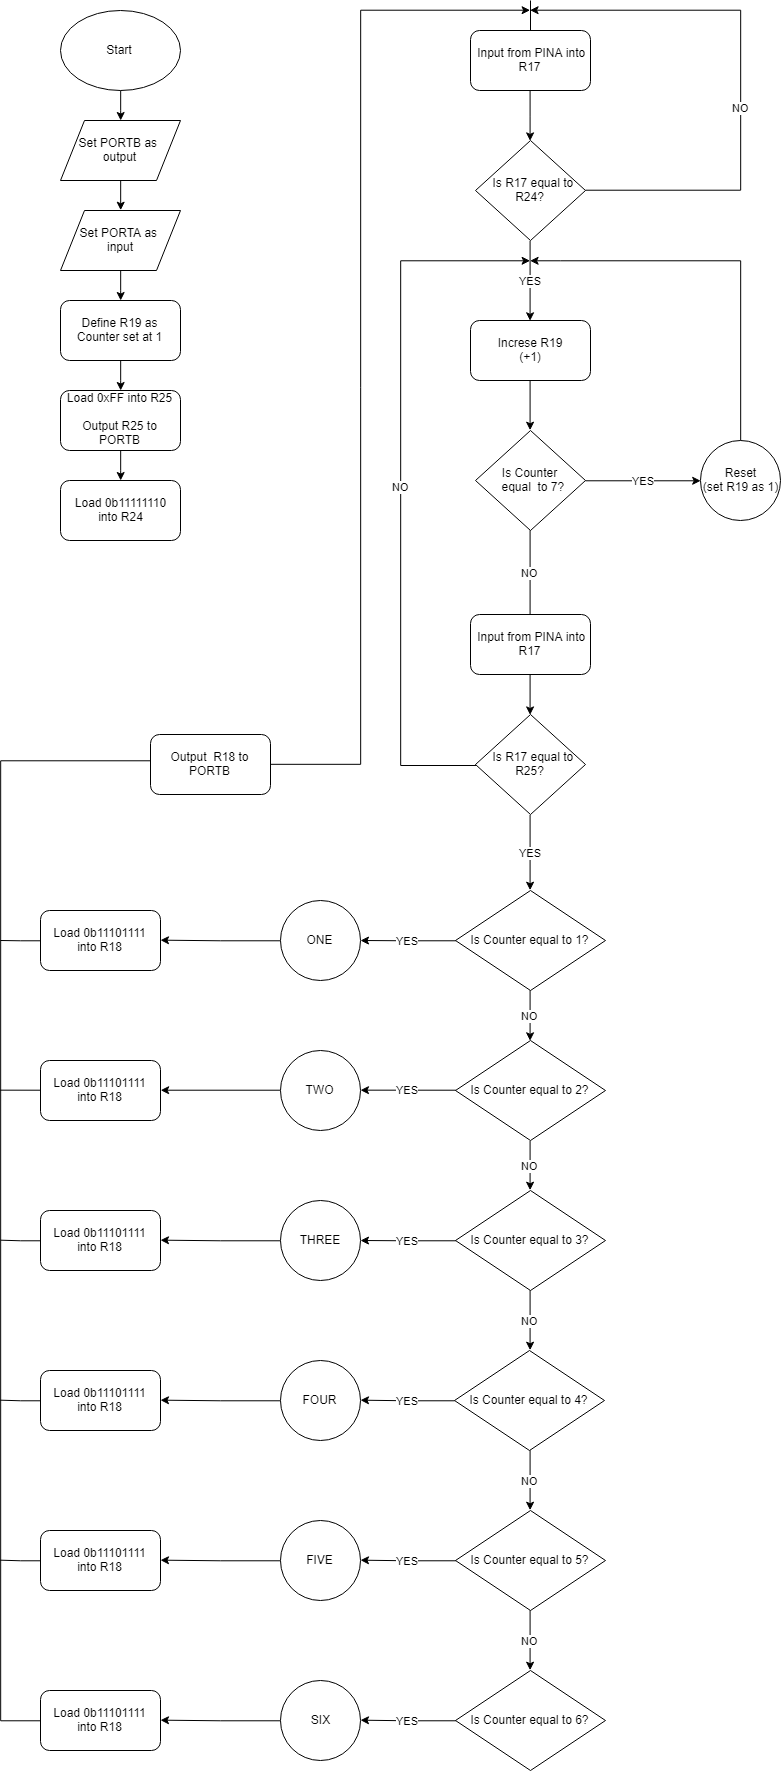
\includegraphics[scale=0.4]{img/Task2.png}
\end{center}

\newpage
\section{Task 3 - Change counter}
\textit{Write a program that is able to count the number of changes on a switch. As a change we count
when the switch SW0 goes from 0 to 1 and from 1 to 0, we expect therefore positive and negative
edges. We calculate the changes in a byte variable and display its value on PORTB.}

\lstset{style=Asm}
\begin{lstlisting}
;>>>>>>>>>>>>>>>>>>>>>>>>>>>>>>>>>>>>>>>>>>>>>>>>>>>>>>>>>>>
; 1DT301, Computer Technology I
; Date: 2016-09-15
; Author:
; Loic GALLAND
; Leonardo PEDRO
;
; Lab number: 2
; Title: Subroutines
;
; Hardware: STK600, CPU ATmega2560
;
; Function:Program that count every time the switch number 0 is pressed or released. it will show the count with binary code on the LEDs
;
; Input ports: PORTA will be used as input to get information from the switches
;
; Output ports: PORTB will be used as output to light up the LEDs
;
; Subroutines: None needed in this Task
; Included files: m2560def.inc
;<<<<<<<<<<<<<<<<<<<<<<<<<<<<<<<<<<<<<<<<<<<<<<<<<<<<<<<<<<<
.include "m2560def.inc"

ldi r16, 0xFF ;setting up the data direction register port B
out DDRB, r16 ;Set port B as output

ldi r16,0x00	;setting up the data direction register PORTA
out DDRA, r16	;Set PORTA as input

ldi r25, 0	;Counter 

ldi r17, 0b11111111
out PORTB, r17	;Turn off all the LEDs

ldi r18, 0b11111110	;Desired switch binary code

my_loop:
	in r19, PINA	;Check input from swiches
	cp r18,r19	;compare input with desired switch
	breq counter_when_switch_pressed
rjmp my_loop
;The switch is now pressed
counter_when_switch_pressed:
	inc r25	;increase r25 by 1
	mov r20,r25	;Copy r25 into r20
	com r20	;COM it to make it show the binary code, so that when the light turns on it represent the 1 of binary code
	out portB,r20	;Show the result on the LEDs
		loop:	;To check when the switch will be release
			in r19,PINA	;Get information from the switches 
			cp r19,r17	; Compare input with desired switch
			breq counter_when_switch_released
		rjmp loop
;Go here when switch is released
counter_when_switch_released:
	inc r25	;Increase r25 by 1
	mov r20,r25	;Copy register r25 into r20
	com r20	;One's Complement of r20 to get the count in binary number to light up the LEDs
	out portB,r20	;Show the result on the LEDs by light them
	rjmp my_loop
\end{lstlisting}

\newpage
This is the flowchart of the task 3:
\begin{center}
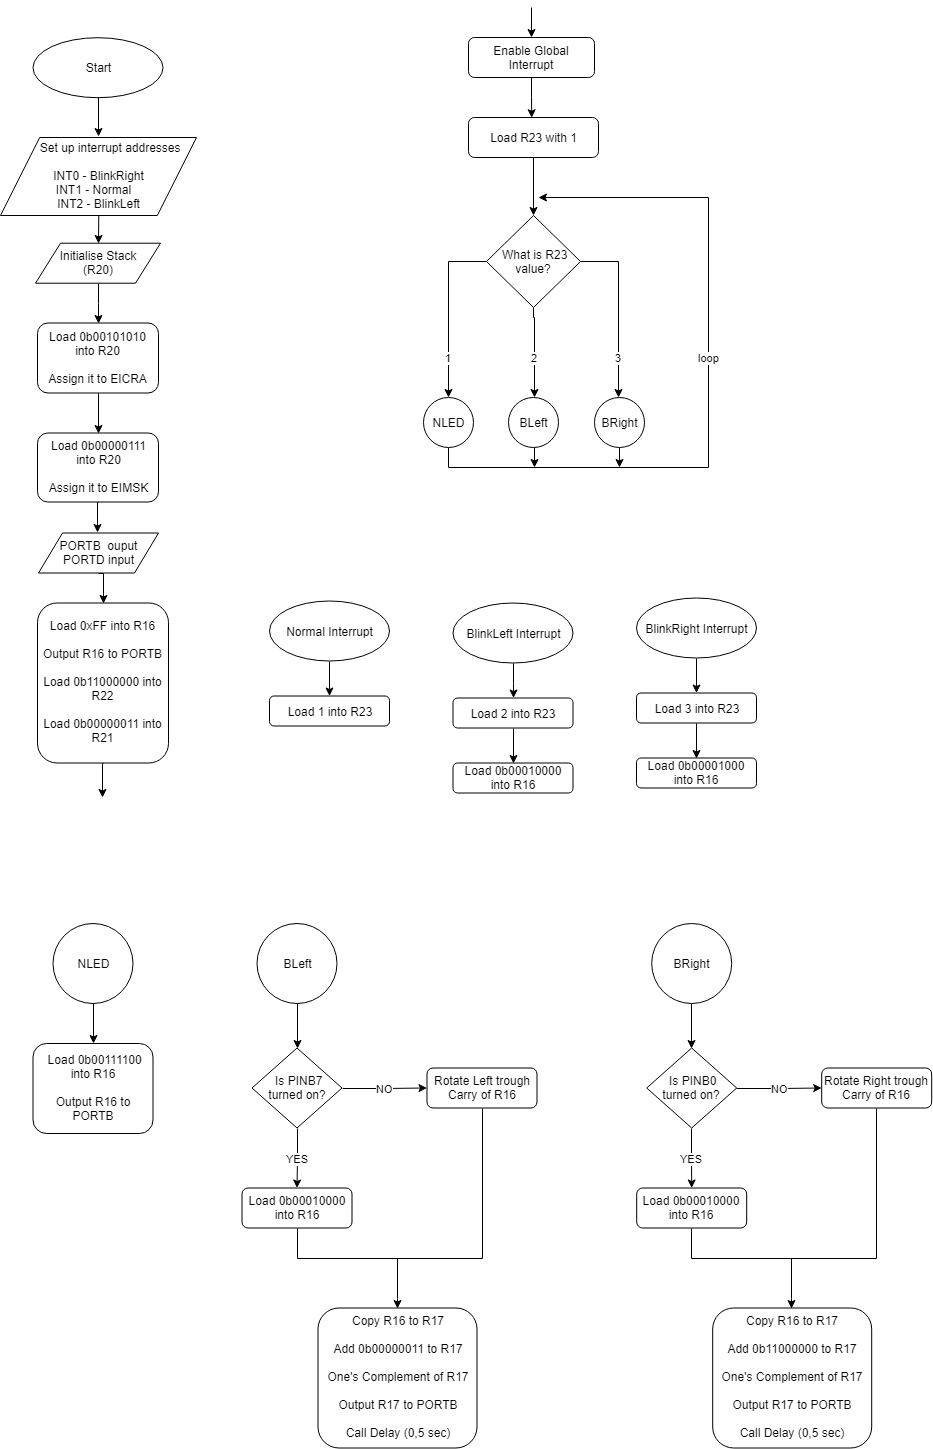
\includegraphics[scale=0.8]{img/TASK3.png}
\end{center}

\newpage
\section{Task 4 - Delay subroutine with variable delay time}

\lstset{style=Asm}
\begin{lstlisting}
;>>>>>>>>>>>>>>>>>>>>>>>>>>>>>>>>>>>>>>>>>>>>>>>>>>>>>>>>>>>
; 1DT301, Computer Technology I
; Date: 2016-09-15
; Author:
; Loic GALLAND
; Leonardo PEDRO
;
; Lab number: 2
; Title: Subroutines
;
; Hardware: STK600, CPU ATmega2560
;
; Function: Create a Delay that can be changed depensidng on what the user chooses
;
; Input ports: NO input will be needed 
;
; Output ports: PORTB will be used as output to control the LEDs
;
; Subroutines: Used to create the Delay
; Included files: m2560def.inc
;<<<<<<<<<<<<<<<<<<<<<<<<<<<<<<<<<<<<<<<<<<<<<<<<<<<<<<<<<<<
.include "m2560def.inc"
.equ INPUT= 1000	;Used this to set how long is the delay.

; Initialize SP, Stack Pointer
ldi r20, HIGH(RAMEND) ; R20 = high part of RAMEND address
out SPH,R20 ; SPH = high part of RAMEND address
ldi R20, low(RAMEND) ; R20 = low part of RAMEND address
out SPL,R20 ; SPL = low part of RAMEND address

ldi r16, 0xFF ;setting up the data direction register port B
out DDRB, r16 ;Set port B as output

ldi r21, 0b11111111; inital LED state
out portB, r21	;Light up the corresponding LEDs
mov r17, r21	;Copy the register r21 into r17
ldi r22, 0xFF	;Desired state of the LEDs
ldi r23, 0b11111110	;Iniatialize the LEDs
RC_loop:
	out portB, r17	;Light up the corresponding LEDs
	rol r17	;Rotate all the bits to the left
	CALL Delay		;Delay of 0.5s
	cp r17, r22		;Compare the LEDs with the desired one
	breq RC_light
rjmp RC_loop

RC_light:
	rol r17	;rol again without output to skip the state where all the LEDs are turn off 
	out portB, r17	;Show corresponding LEDs to PORTB
	rjmp RC_loop	;Jump back to the main loop

Delay:
	ldi r24, low(INPUT)	;Use r24 and r25 to create a 16bit register. Set r24 with the Low end
	ldi r25, high(INPUT)	;And r25 for the high end of the register
	wait_milliseconds:	;Will go into this loop the amount of time we have 
		call ms_delay	;Call method ms_delay that will last only 1ms
		sbiw r25:r24,1	;Reduce the count by 1 of the 16bits register
		cpi r25, high(0)	;Compare when the r25 is equal and therefore the 
		breq reset		;Delay is finished
	rjmp wait_milliseconds
reset:
RET	;to make it go back to the loop "RC_loop"

ms_delay:	;Delay of 1ms
	; Generated by delay loop calculator
	; at http://www.bretmulvey.com/avrdelay.html
	; Delay 1 000 cycles
	; 1ms at 1 MHz
	ldi  r18, 2
	ldi  r19, 75
L1: dec  r19
	brne L1
	dec  r18
	brne L1
	rjmp PC+1
RET
\end{lstlisting}

\newpage
This is the flowchart of the task 4:
\begin{center}
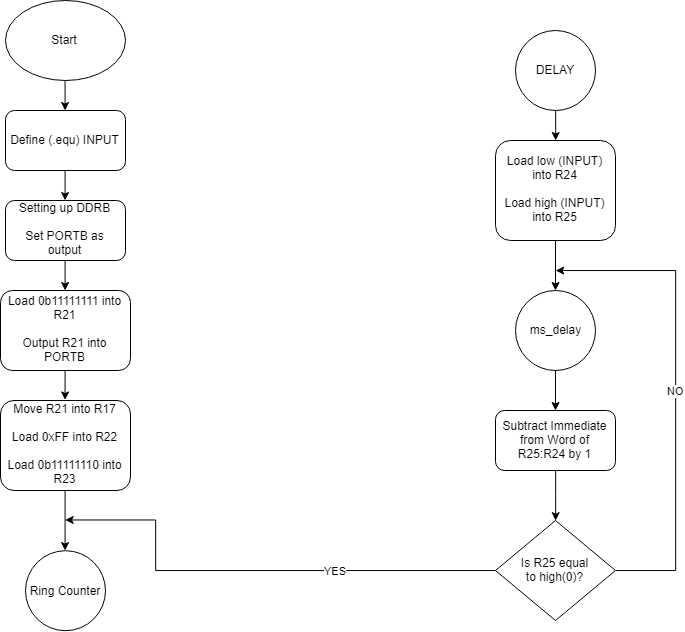
\includegraphics[scale=0.7]{img/Task4.png}
\end{center}
% Prints your bibliography database xxx.bib
\bibliographystyle{IEEEtran}
\bibliography{ref.bib}

\end{document}
